\chapter{Módulo Mobile}
\noindent
Este capítulo tem o objetivo de abordar o 2º módulo do projeto, o módulo \textit{mobile}. De maneira geral, ele é o responsável por retirar a fotografia da turma, captar os dados relativos ao código identificador, tempo de aula e, por fim, enviar toda a informação para o servidor e no servidor realizar o recebimento. O servidor conforme apresentado anteriormente, será responsável pela análise da foto. 
\section{Conceito Geral do módulo}
\noindent
Desenvolvido para plataforma Android, a aplicação deverá proporcionar ao usuário, professor, uma interface simples e intuitiva para a realização das tarefas propostas. O professor deve ser capaz de realizar a seleção de uma fotografia, já salva na galeria ou tirada no próprio momento, completar o registro de informações essenciais e realizar o posterior envio. O diagrama de atividades pode ser visto na figura \ref{fig:figura80}
\begin{figure}[!ht]
	\centering
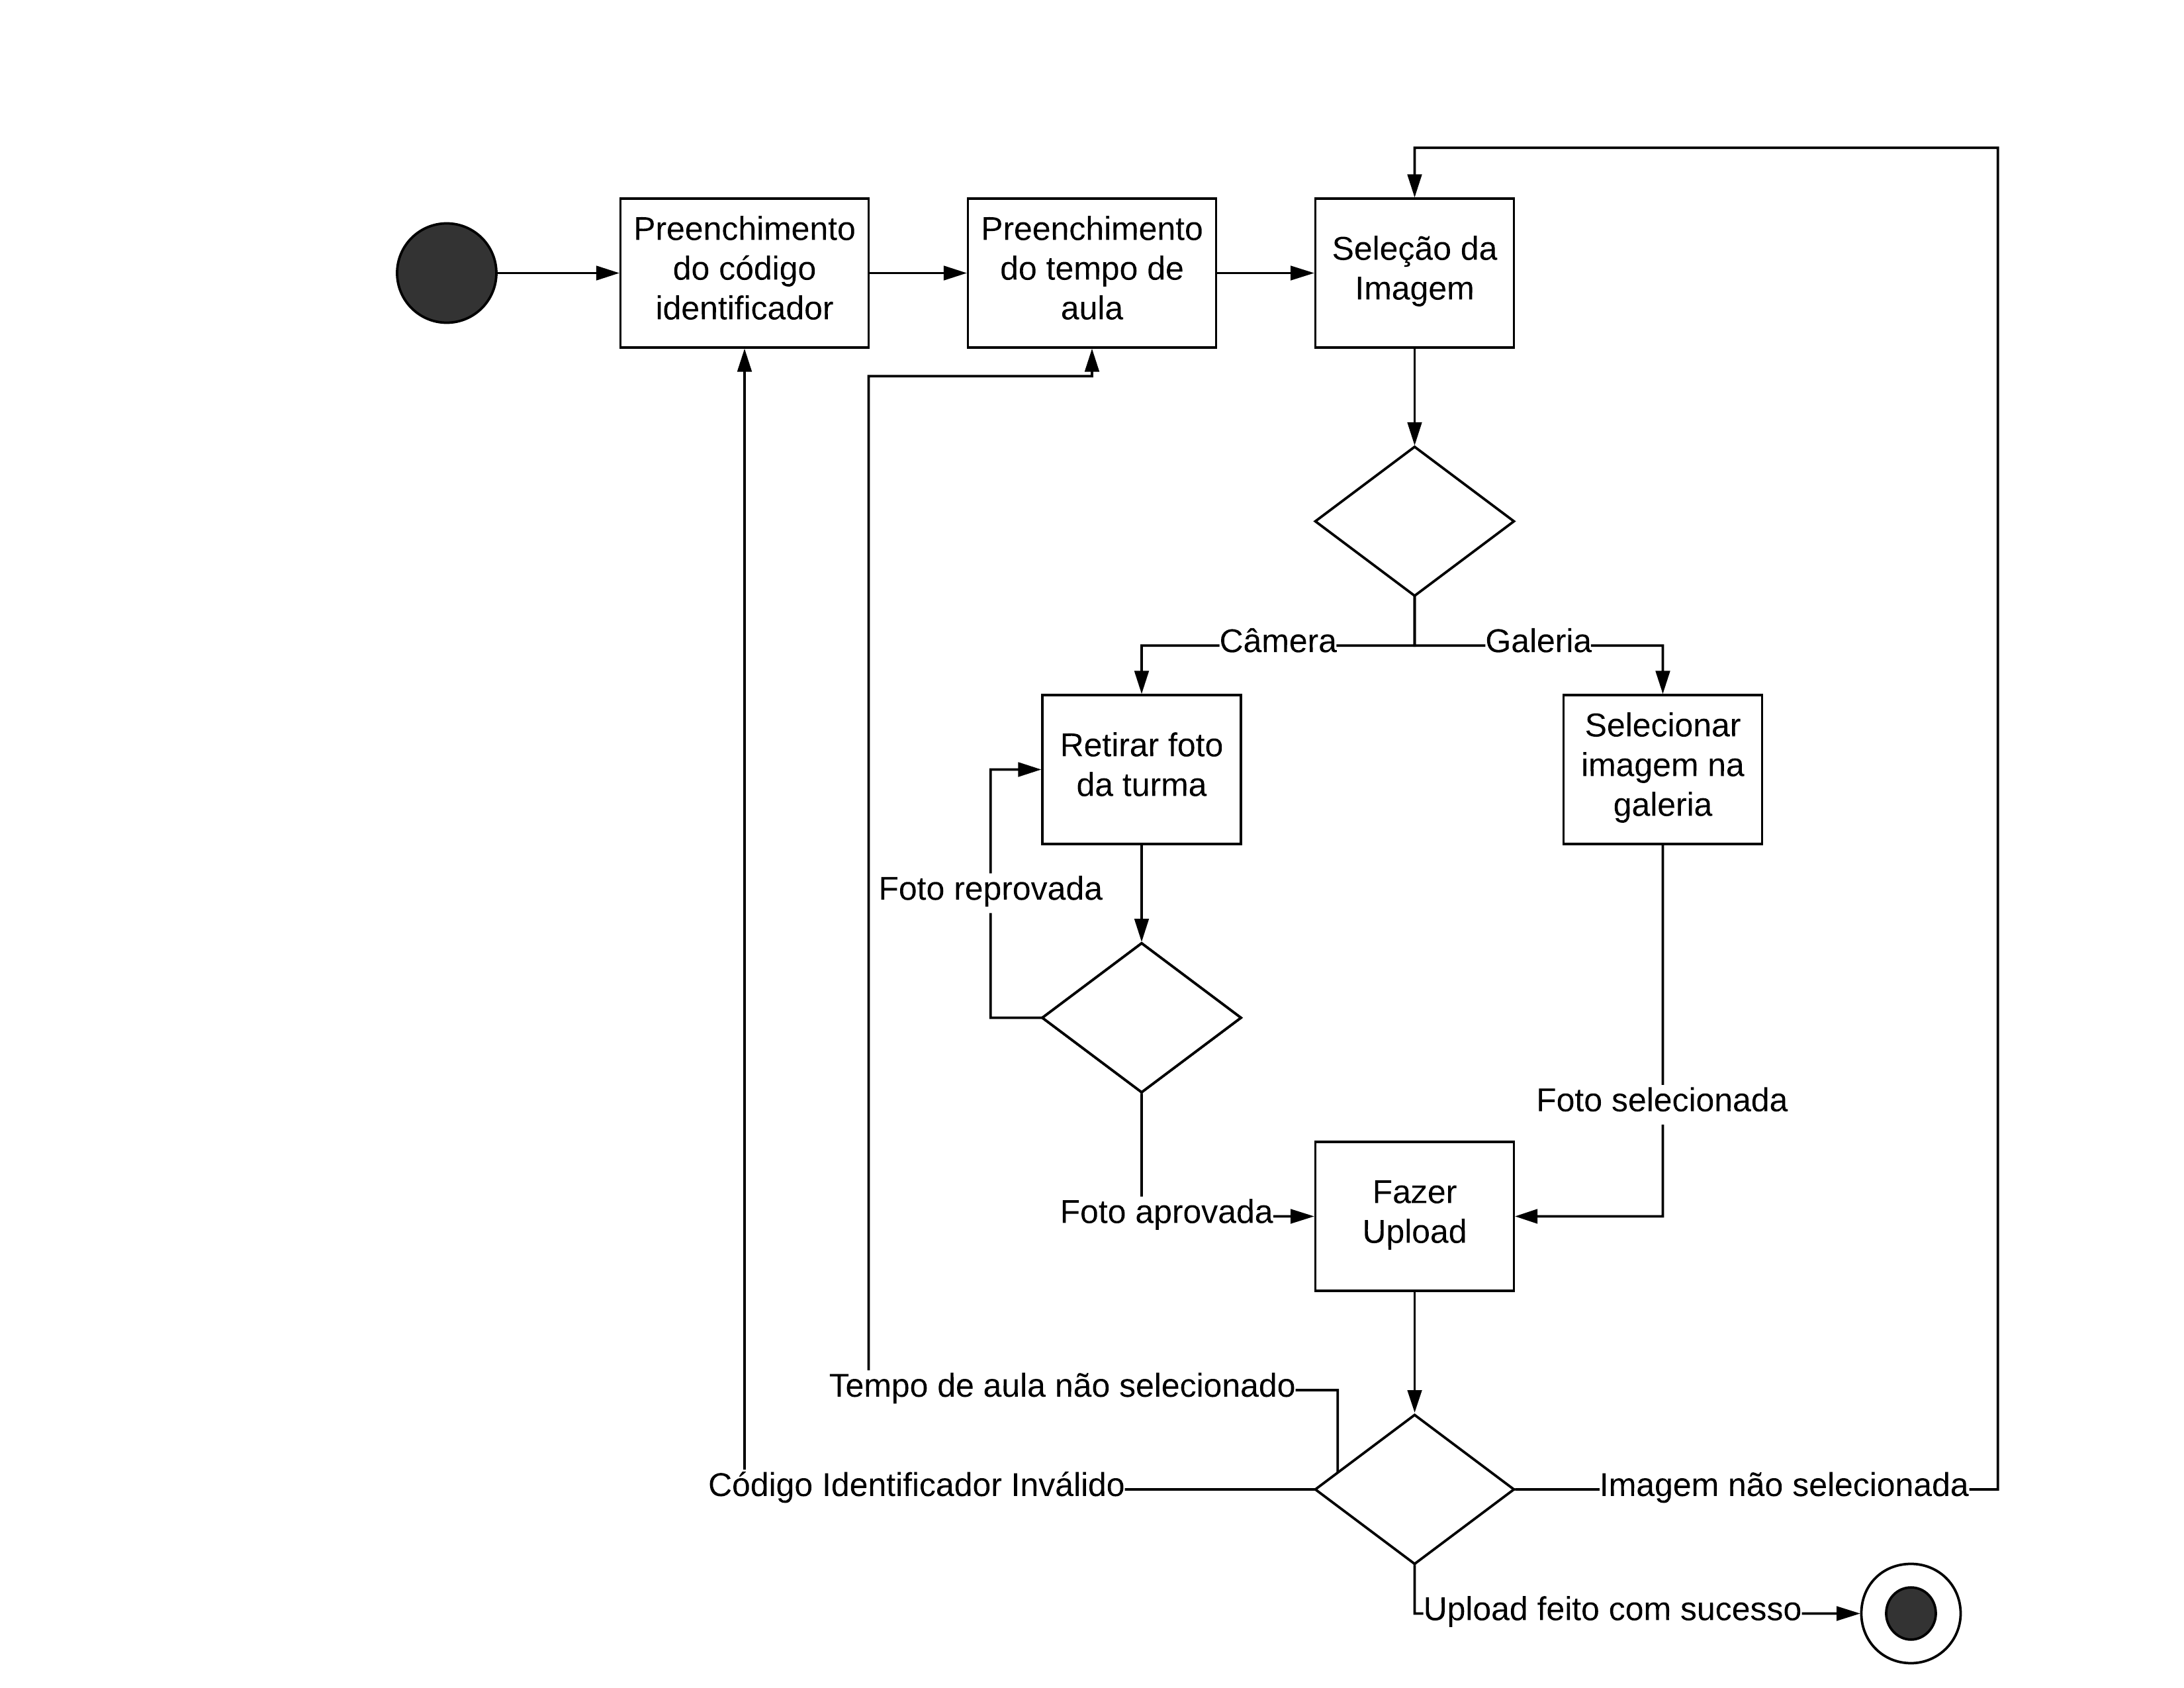
\includegraphics[width=1.0\textwidth]{diagrama_atividades.png}
	\caption{Diagrama de atividades}
	\label{fig:figura80}
\end{figure}

\section{Plataforma Android}
Android é uma plataforma móvel baseada em Linux, cujo desenvolvimento propunha já desde os primórdios um desenvolvimento sob padrão aberto, ou seja, um padrão que está disponível para o público \citep{Android1}. O projeto foi desenvolvido pelo consórcio de empresas de tecnologias Open Handset Alliance, contendo gigantes do mercado como Google, Sony, Samsung e outras operadoras de telefonia e fabricantes de dispositivos \citep{Android2}.  A pilha de software do Android pode ser vista em detalhes na figura \ref{fig:figura58b}, que mostra a maioria dos componentes da plataforma Android \citep{Android1}.

\begin{figure}[!ht]
	\centering
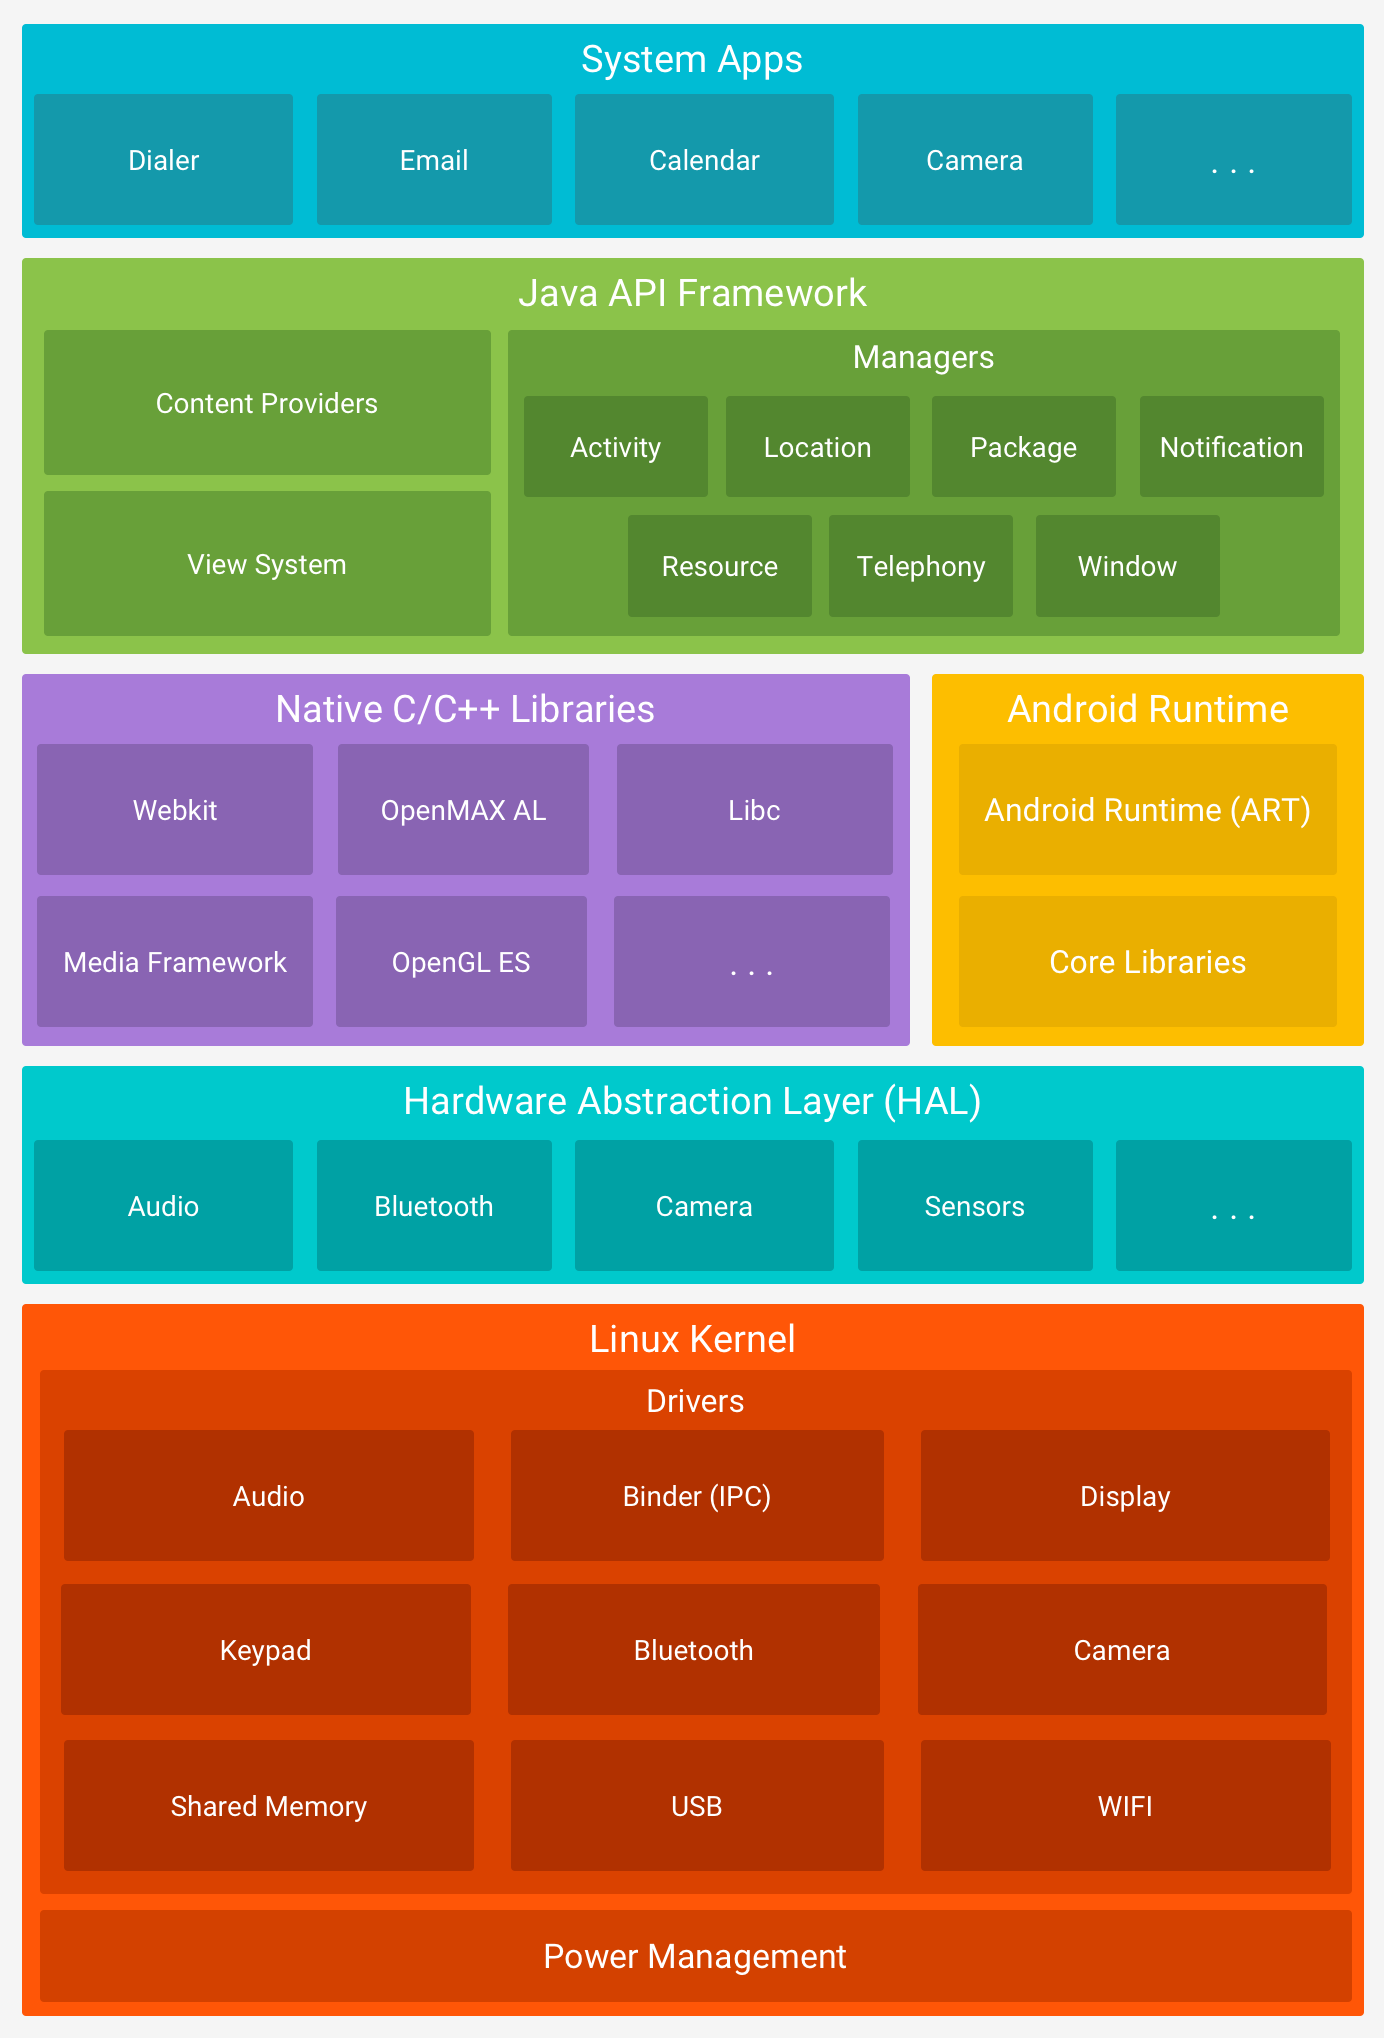
\includegraphics[width=0.6\textwidth]{arquitetura_android.png}   
	\caption{Pilha de software do Android v. abril 2018}\citep{Android1}
	\label{fig:figura58b}
\end{figure}



A equipe de desenvolvedores lideradas por Andy Rubinera criou no android a capacidade de acessar informações por meio de poucos toques extremamente intuitivos. Uma das grandes vantagens é tornar o sistema acessível para o usuário casual, ou seja, utilizadores que não possuem grande conhecimento tecnológico. De forma fluida, portanto, a plataforma permite a utilização dos mais diversos aplicativos sem demandar um processo de reaprendizado custoso por parte do usuário, visto que as características do dispositivos presente nos aplicativos torna familiar a experiência mesmo se tratando de novos aplicativos \citep{Android3}.

A possibilidade de usar componentes já prontos intrínsecos ao sistema operacional, como a interface de controle da câmera fotográfica, diminui o custo de desenvolvimento para o software em questão ao se escolher a plataforma Android, além de aumentar de forma relevante a qualidade do produto desenvolvido, já que os componentes reutilizados dentro da aplicação já foram exaustivamente testados antes de serem homologados e disponibilizados para uso. A utilização da câmera fotográfica através da aplicação pode ser vista na figura \ref{fig:figura59}.

Todos esses fatores fizeram com que a plataforma Android dominasse o mercado de maneira avassaladora. Segundo pesquisa liderada pela corporação IDC, International Data Corporation, no primeiro quarto de ano de 2017, a plataforma estava presente em 85\% dos aparelhos mobile ao redor do mundo, justificando o rótulo de plataforma mais popular do mundo, presente até mesmo no site oficial Android \citep{Android4} \citep{Android5}. No Brasil, a hegemonia é ainda mais significante, segundo dados da empresa Kantar, tendo alcançado 93\% do mercado nacional em março de 2018 \citep{Android6}.

Esses dados corroboram a escolha da plataforma para construção do aplicativo, que busca ser o mais acessível possível.


\subsection{Ambiente de desenvolvimento}
Buscando tornar o aplicativo o mais acessível possível, este foi desenvolvido tendo como base a API 15: Android 4.0.3 (\textit{IceCreamSandwich}), sendo compatível com quase a totalidade de aplicativos existentes, segundo estatísticas do próprio Android Studio.
%\begin{figure}[!ht]
%	\centering
%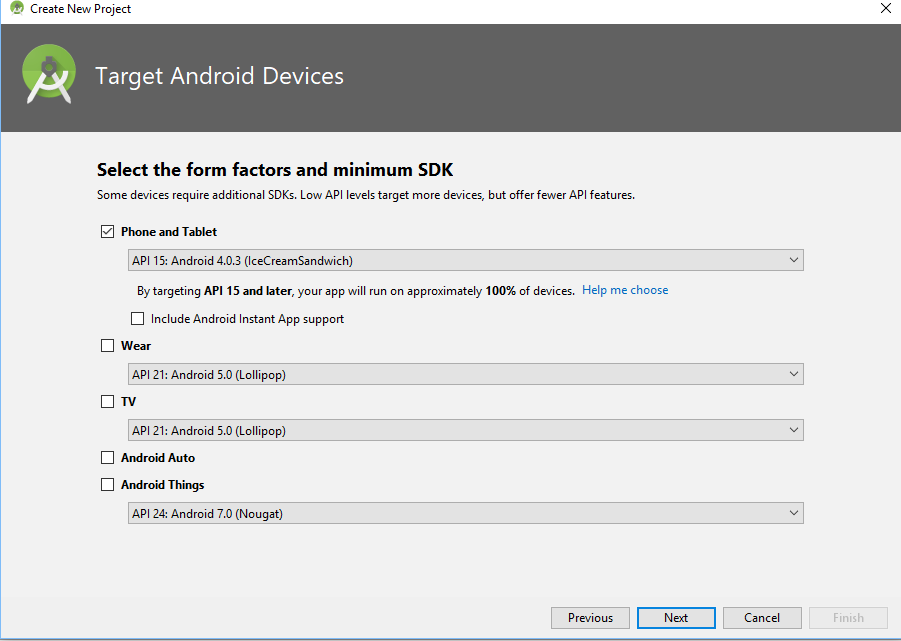
\includegraphics[width=1.0\textwidth]{target_devices.png}   
%	\caption{Dispositivos compatíveis}
%	\label{fig:figura60}
%\end{figure}

Utilizou-se a versão estável mais atual do Android Studio, visando tornar o código compatível com os recursos mais recentes oferecidos por esse ambiente de desenvolvimento. A figura \ref{fig:figura61} contém as informações sobre a versão utilizada, contruída em 4 de Junho de 2018.
\begin{figure}[!ht]
	\centering
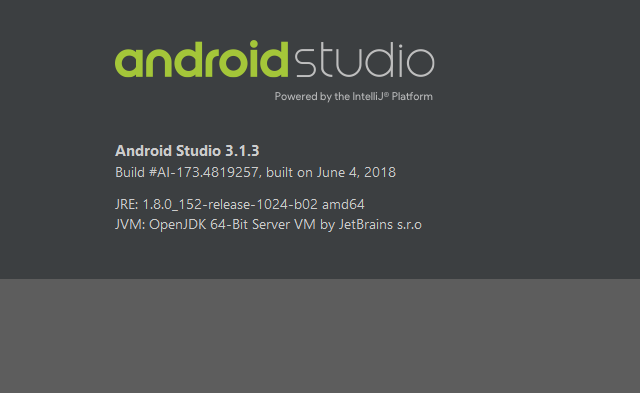
\includegraphics[width=0.55\textwidth]{versao_android.png}   
	\caption{Versão Android}
	\label{fig:figura61}
\end{figure}

\subsection{Linguagem de programação}
A linguagem de programação utilizada foi Java, utilizada pelo Android Software Development Kit, SDK. A utilização do SDK é a escolha recomendada oficialmente pela Google, visto que a Android Native Development Kit, NDK, só é aconselhável caso verdadeiramente se necessite ganhar maior desempenho, já que se rodaria a aplicação diretamente no processador \citep{Android7}. Esse ganho extra de desempenho, que aumentaria a complexidade do código, não é justificável visto que o processamento exigido durante toda a aplicação é extremamente reduzido. Além disso, ao utilizar o SDK se tem a garantia de portabilidade de dispositivo independentemente da arquitetura do processador, corroborando com a tentativa de tornar o aplicativo o mais acessível quanto possível \citep{Android8}.


\subsection{Dispositivos de teste}
Os dispositivos, ilustrados pelas figuras \ref{fig:figura62} e \ref{fig:figura63}, foram utilizados neste projeto para
a realização de testes da aplicação desenvolvida.

\begin{figure}[!ht]
	\centering
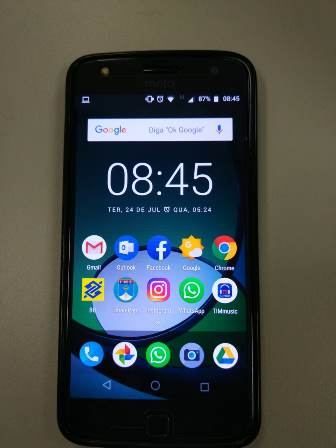
\includegraphics[width=0.25\textwidth]{img/moto_z_play.jpeg}   
	\caption{MOTO Z Play - Processador Snapdragon™ 625 Qualcomm® 3GB de RAM}
	\label{fig:figura62}
\end{figure}


\begin{figure}[!ht]
	\centering
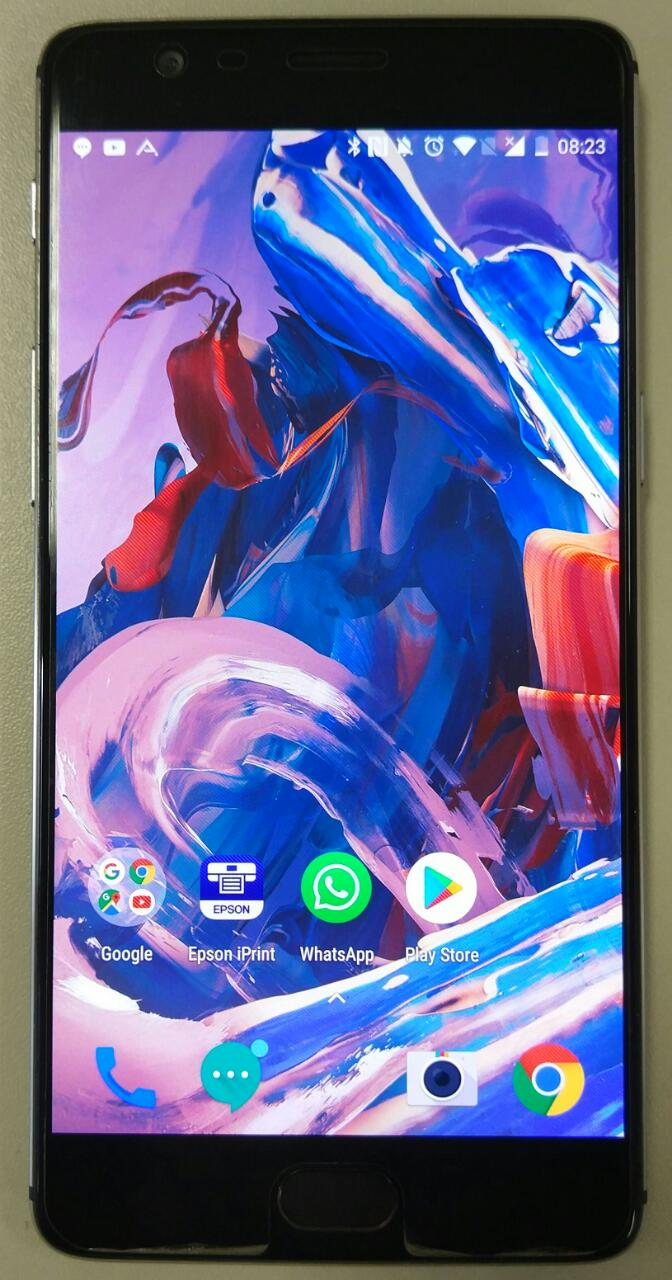
\includegraphics[width=0.15\textwidth]{img/Oneplus3.jpg}
	\caption{One Plus 3 - Processador Snapdragon™ 820 Qualcomm® 6GB de RAM}
	\label{fig:figura63}
\end{figure}

Nenhuma diferença de desempenho foi observada ao utilizar a aplicação nos diferentes dispositivos. Ambos aparelhos foram testados utilizando o Android 8.0.0. 

A única funcionalidade da aplicação verdadeiramente dependente de alguma característica do dispositivo é o acionamento da câmera, cuja utilização através da aplicação só pode ser executada caso o dispositivo possua câmera. Colocou-se uma verificação que libera o clique de acesso a câmera apenas para aqueles dispositivos que possuem o hardware. Devido a incapacidade de tirar fotos caso a câmera não exista, a verificação impede que o aplicativo gere um erro crítico. Ainda assim, contudo, é possível realizar envio completo das informações para retirada de faltas mesmo em um celular sem câmera, bastando utilizar uma imagem salva na galeria. A utilização da câmera através da aplicação pode ser revista na figura \ref{fig:figura59}, já mencionada anteriormente.

\begin{figure}[!ht]
	\centering
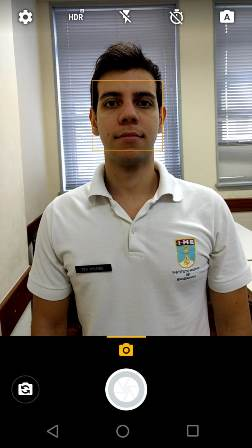
\includegraphics[width=0.2\textwidth]{img/camera_1.jpeg}   
	\caption{Utilização da câmera através da aplicação}
	\label{fig:figura59}
\end{figure}

\newpage
\section{A aplicação}
O objetivo da aplicação, conforme descrito no início do capítulo é garantir o preenchimento de informações necessárias para a retirada de faltas de maneira fluída e intuitiva. A figura \ref{fig:figura64} mostra a tela inicial da aplicação.


\begin{figure}[!ht]
	\centering
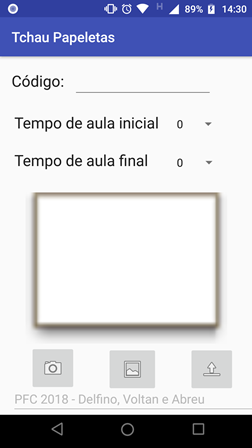
\includegraphics[width=0.3\textwidth]{Tela_Inicial_Aplicacao.png}   
	\caption{Tela inicial da aplicação}
	\label{fig:figura64}
\end{figure}

\subsection{Preenchimento do código identificador}
O preenchimento do código identificador, figura \ref{fig:figura65} ocorre ao clicar-se sobre o campo destinado para o mesmo, quando abrir-se-á o teclado e o professor poderá digitar a referência à turma e à matéria por ele ministrada. No exemplo a seguir, ilustradro na figura \ref{fig:figura66}, tem-se turma1 e disciplina Redes1, gerando o código identificador "turma1.Redes1". 

\begin{figure}[!ht]
	\centering
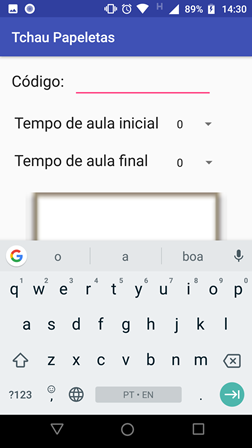
\includegraphics[width=0.3\textwidth]{Preenchimento_c_digo.png}   
	\caption{Teclado para digitação}
	\label{fig:figura65}
\end{figure}

\begin{figure}[!ht]
	\centering
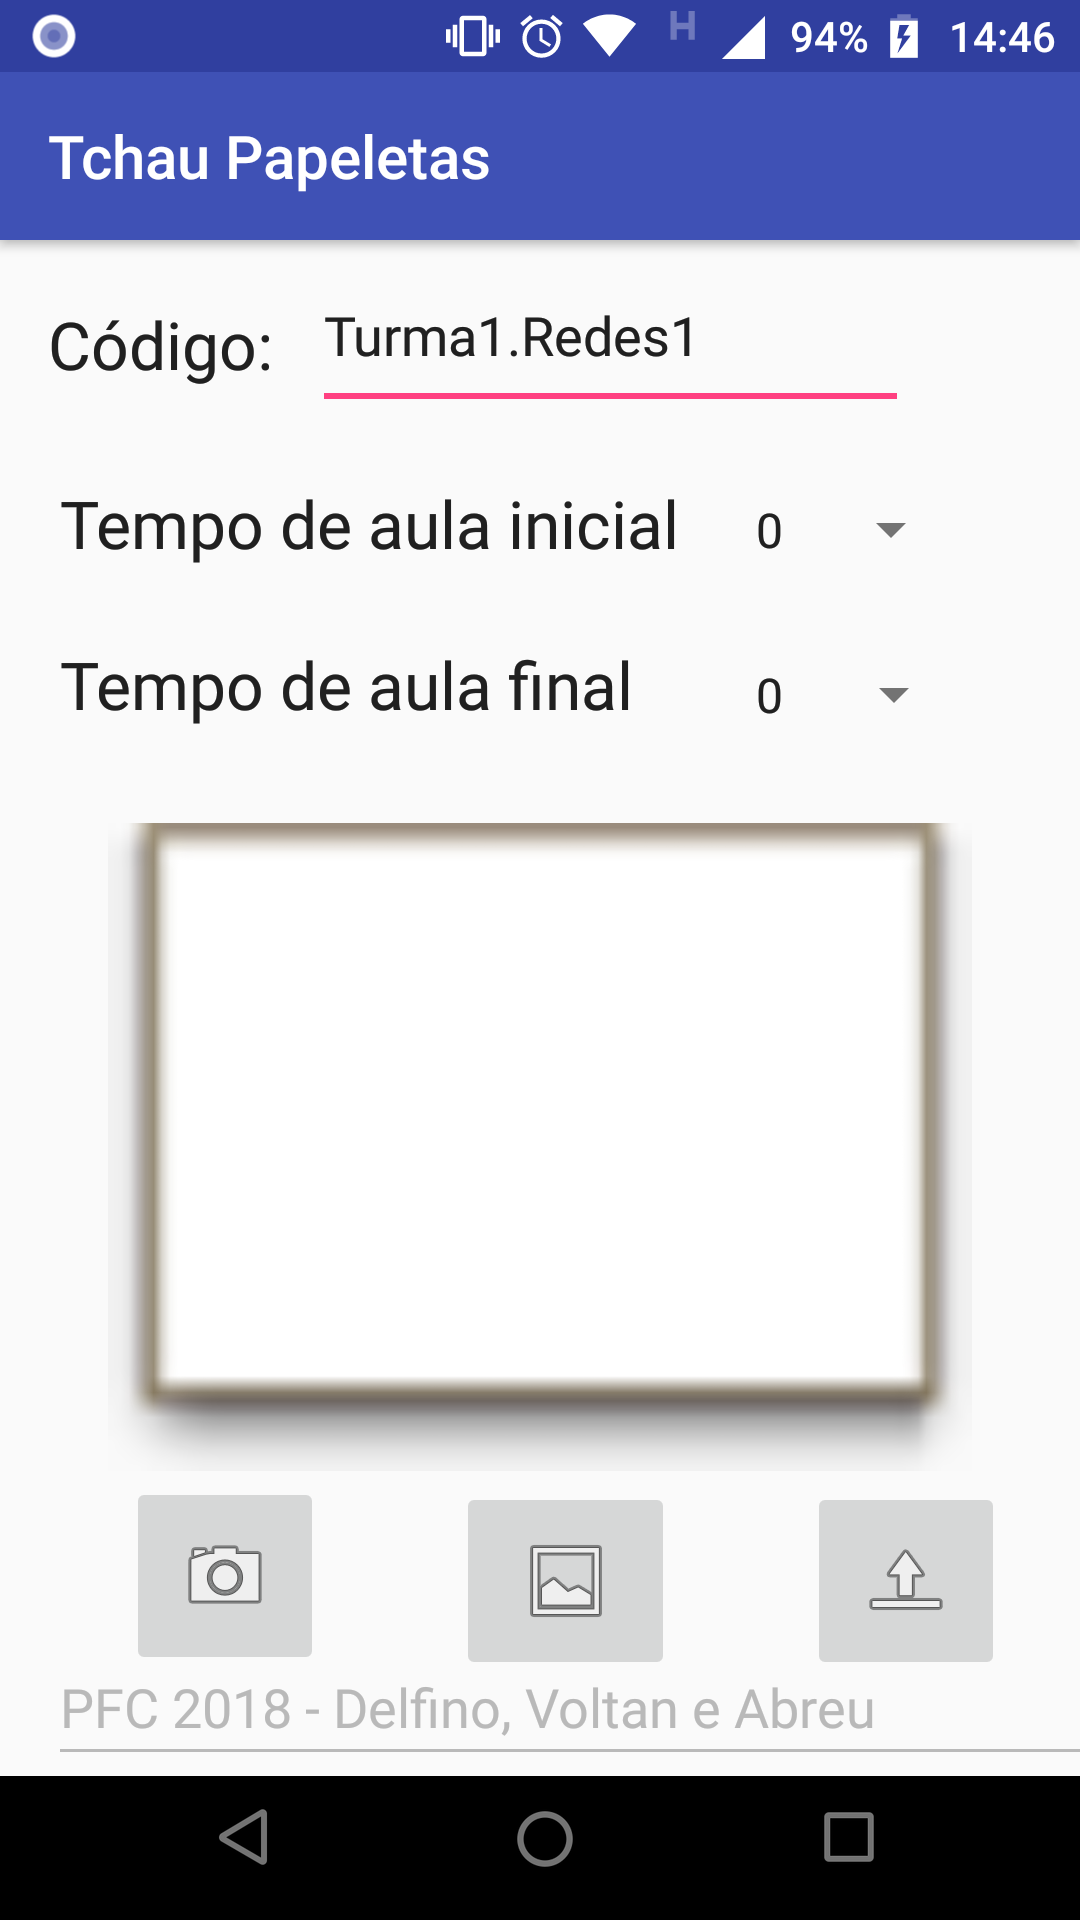
\includegraphics[width=0.3\textwidth]{C_digo_preenchido.png}   
	\caption{Código preenchido}
	\label{fig:figura66}
\end{figure}

No atual momento de desenvolvimento optou-se por deixar esse campo com preenchimento livre de tal forma a possibilitar utilização por qualquer turma e qualquer disciplina, não o limitando a escolhas restritas das disciplinas de alguma seção de ensino, por exemplo. O objetivo é tornar o aplicativo compatível com futuras aplicações e diferentes turmas e disciplinas.


\subsection{Preenchimento do tempo de aula}
O preenchimento dos tempos de aula ocorre clicando sobre os tempos de aula correspondentes, figura \ref{fig:figura57b}. Como os tempos de aula possíveis já estão previamente definidos, optou-se por realizar o preenchimento desse campo através de um controle giratório. Basta clicar na opção desejada para o tempo de aula, quando abrir-se-ão opções de tempos do 1 ao 11, intervalo de horário máximo segundo quadro de horários vigente no IME. 

\begin{figure}[!ht]
	\centering
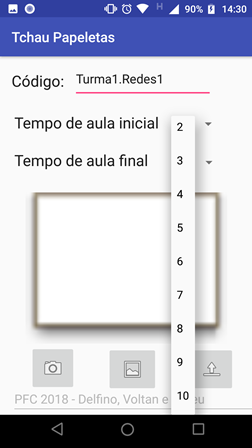
\includegraphics[width=0.3\textwidth]{preenchimento_tempo_de_aula.png}   
	\caption{Preenchimento Tempo de aula}
	\label{fig:figura57b}
\end{figure}

\subsection{Aquisição da imagem}
A aquisição da imagem pode ser feita de duas maneiras diferentes:

• Por meio do acesso à galeria de imagens do dispositivo; ou

• Por meio da captura de uma imagem através da câmera do dispositivo.

\subsubsection{Câmera}
Para iniciar abertura da câmera basta clicar sobre o ícone da câmera. A interface de câmera do sistema operacional Android vigente então abrirá, permitindo a retirada de fotos já familiar ao usuário. Após retirada da foto, o usuário terá opção de confirmar ou rejeitar a foto obtida, figura \ref{fig:figura59b}. Exibir-se-á na tela inicial da aplicação, então, a foto tirada, caso essa tenha sido aprovada pelo usuário.

%\begin{figure}[!ht]
%	\centering
%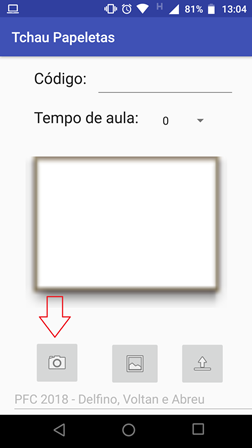
\includegraphics[width=0.3\textwidth]{Icone_1.png}   
%	\caption{Ícone câmera}
%	\label{fig:figura68}
%\end{figure}

\begin{figure}[!ht]
	\centering
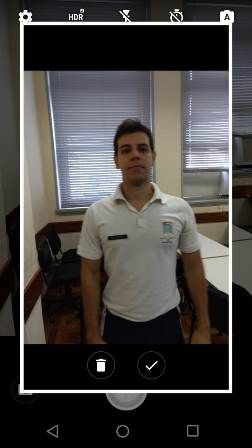
\includegraphics[width=0.3\textwidth]{img/camera_2.jpeg}   
	\caption{Aguardando aprovação da foto tirada}
	\label{fig:figura59b}
\end{figure}

%\begin{figure}[!ht]
%	\centering
%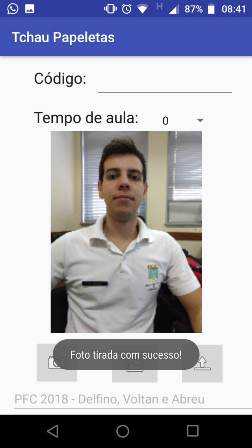
\includegraphics[width=0.3\textwidth]{img/camera_3.jpeg}   
%	\caption{Foto Tirada com sucesso}
%	\label{fig:figura69}
%\end{figure}

\subsubsection{Galeria}
Para iniciar a escolha de foto através da galeria basta clicar sobre o ícone da galeria. A interface de galeria do sistema operacional Android vigente então abrirá, permitindo a escolha de fotos já familiar ao usuário, conforme ilustrado na figura \ref{fig:figura71}. Exibir-se-á na tela inicial da aplicação, então, a foto selecionada pelo usuário. Um exemplo de exibição da foto escolhida na tela inicial da aplicação pode ser vista na figura \ref{fig:figura81}. 
%\begin{figure}[!ht]
%	\centering
%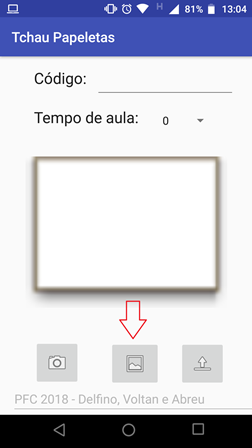
\includegraphics[width=0.3\textwidth]{img/Icone_2.png}   
%	\caption{Ícone galeria}
%	\label{fig:figura70}
%\end{figure}

\begin{figure}[!ht]
	\centering
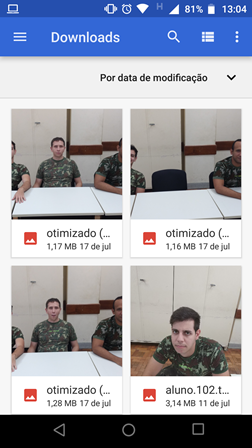
\includegraphics[width=0.3\textwidth]{img/Galeria.png}  
	\caption{Seleção da foto a partir da galeria}
	\label{fig:figura71}
\end{figure}

\begin{figure}[!ht]
	\centering
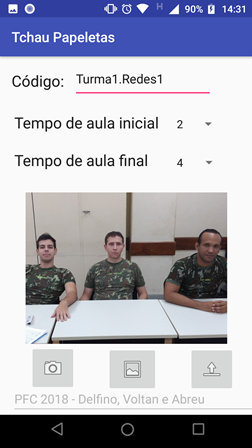
\includegraphics[width=0.3\textwidth]{img/foto_selecionada_com_sucesso.png}  
	\caption{Foto selecionada com sucesso}
	\label{fig:figura81}
\end{figure}

\subsection{Upload para o servidor}
Para enviar todos os dados para o servidor, basta clicar no ícone de \textit{upload}. A aplicação enviará toda a informação coletada caso todos os campos tenham sido preenchidos de maneira adequada. Na impossibilidade dos dados serem aprovados, a aplicação notificará o usuário por meio de notificações qual campo está impossibilitando o sucesso da execução, conforme mostram as figuras \ref{fig:figura73}, \ref{fig:figura74} e \ref{fig:figura75}.

%\begin{figure}[!ht]
%	\centering
%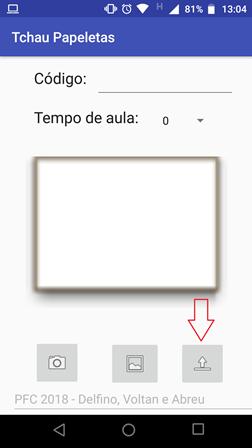
\includegraphics[width=0.3\textwidth]{img/Icone_3.png}   
%	\caption{Ícone upload}
%	\label{fig:figura72}
%\end{figure}
\begin{figure}[!ht]
	\centering
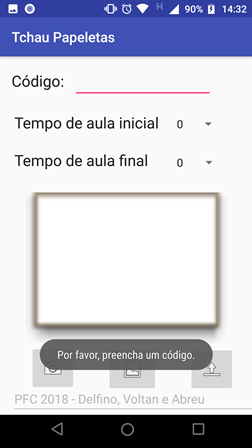
\includegraphics[width=0.3\textwidth]{toast_codigo.png}   
	\caption{Erro no preenchimento do código}
	\label{fig:figura73}
\end{figure}

\begin{figure}[!ht]
	\centering
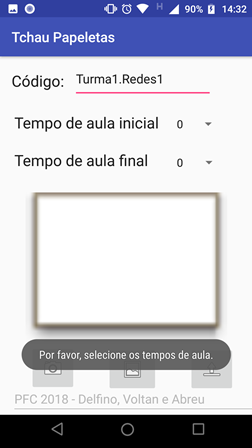
\includegraphics[width=0.3\textwidth]{toast_tempo_de_aula.png}   
	\caption{Erro no preenchimento do tempo de aula}
	\label{fig:figura74}
\end{figure}

\begin{figure}[!ht]
	\centering
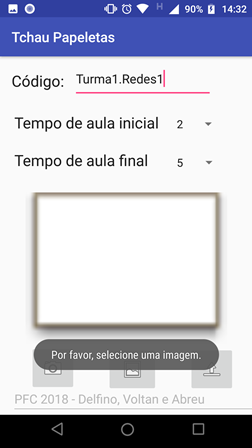
\includegraphics[width=0.3\textwidth]{toast_imagem.png}   
	\caption{Erro na seleção de Imagem}
	\label{fig:figura75}
\end{figure}

Caso todas as informações tenham sido preenchidas corretamente, notificar-se-á o usuário do upload feito de maneira correta, de maneira temporária e também de maneira persistente, figura \ref{fig:figura76}. Além disso, não mais se exibirá a foto enviada, garantindo a percepção de que aquela foto já foi enviada para o servidor, impedindo assim que o professor persista na tentativa de enviar a mesma informação de maneira duplicada.

\begin{figure}[!ht]
	\centering
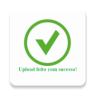
\includegraphics[width=0.3\textwidth]{upload_sucesso.png}   
	\caption{Upload efetuado com sucesso}
	\label{fig:figura76}
\end{figure}
\newpage
%Após conclusão do módulo 3, módulo do banco de dados, estudar-se-á a exibição dos resultados produzidos pelo reconhecimento facial. O módulo 3 também será o responsável pelo armazenamento persistente dessas informações no banco de dados.

No módulo 3, módulo do banco de dados, estudar-se-á a exibição dos resultados produzidos pelo reconhecimento facial. O módulo 3 também será o responsável pelo armazenamento persistente dessas informações no banco de dados.

\section{Especificações do envio}
O envio das informações dar-se-á através de um \textit{socket}, um ponto final de comunicação entre duas máquinas. Para o caso do trabalho em tela, o \textit{smartphone} utilizado pelo professor contendo a aplicação instalada, cliente, e o computador contendo o servidor. 

Utilizar-se-á o protocolo TCP para a transmissão. A escolha pela não utilização do \textit{DatagramSocket}, que utilizaria o protocolo UDP, deu-se fundamentalmente pela verificação de envio correto das informações presente na utilização do protocolo TCP \citep{Android10}. Apesar de possibilitar um envio mais rápido, o UDP não é confiável, já que não há garantia que o pacote chegou ao destino da maneira correta, fator impeditivo para seu uso na aplicação em questão \citep{Android9}. Além disso, o ganho de desempenho proporcionado pelo protocolo UDP não é almejado com afinco, visto que enviar-se-á uma foto única, não executando uma transmissão contínua de vídeo, por exemplo, ou seja, não necessita de alta taxa de transmissão \citep{Android9}.

Todas as informações serão enviadas através de uma mensagem única. Para isso, converter-se-á a imagem selecionada. Para isso, criar-se-á o arquivo \textit{Bitmap} da foto da turma especificada, obtida por meio da galeria ou captura de câmera. Tal arquivo será, então, convertido em uma stream de dados, utilizando o formato JPEG para a compressão em um \textit{array} de \textit{bytes}. A escolha do formato JPEG deu-se fundamentalmente por ser permitido definir a qualidade de imagem após conversão, especificada como máxima e permitindo o reconhecimento abordado ao longo do capítulo 4. A informação agora escrita nesse \textit{array} de \textit{bytes} é finalmente convertida em base 64 como uma \textit{string}, para ser adicionada a mensagem enviada pelo \textit{socket}, conforme já mencionado. Por fim, enviar-se-á a mensagem contendo as \textit{strings} de Código, Tempo de aula e Foto convertida em \textit{String}, sendo essas informações separadas por vírgula e incluídas nessa ordem em uma padronização exigida para restauração das imagens uma vez que essas sejam recebidas no Servidor TCP. A decodificação realizada no Servidor TCP exige tal padronização.

\subsection{Cliente TCP}
A execução da tarefa em Android é feita por uma instância da classe \textit{SocketImpl}, através da importação do pacote java.net.Socket. A extensa documentação a respeito da utilização de socket em plataformas android no site oficial de referências, \citep{Android10},  bem como o cumprimento de todos os requisitos propostos para o trabalho foram decisivas para a escolha do método de transmissão.


\subsection{Servidor TCP}
O servidor TCP fará a coleta da informação recebida, separando os dados recebidos e convertendo a imagem recebida para o formato o JPEG, já colocando toda a informação necessária no nome do arquivo criado, seguindo as padronizações especificadas ao longo do módulo 4. 
Optou-se por manter a mesma linguagem de programação utilizada para o desenvolvimento da aplicação Android, buscando manter a coerência dentro do módulo desenvolvido. Assim sendo, toda a aplicação do servidor TCP, que conta com interface gráfica, foi desenvolvida em linguagem de programação Java.

Após clicar em "Iniciar serviço", o servidor TCP atuará de maneira contínua, esperando o recebimento de solicitações feitas através da aplicação e salvando as respectivas imagens com os respectivos códigos associados, conforme ilustrado nas figuras \ref{fig:figura77}, \ref{fig:figura78} e \ref{fig:figura79}. Nenhuma ação é necessária para o recebimento das futuras imagens, sendo o processo de decodificação e posterior registro em disco da imagem recebida com o respectivo nome identificador contínuo.

\begin{figure}[!ht]
	\centering
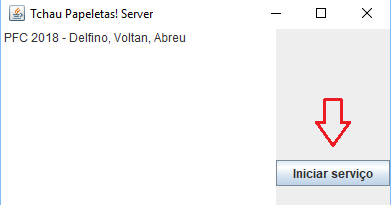
\includegraphics[width=0.5\textwidth]{iniciar_conex_o_1.png}   
	\caption{Iniciando serviço: Passo 1}

	\label{fig:figura77}
\end{figure}
\begin{figure}[!ht]
	\centering
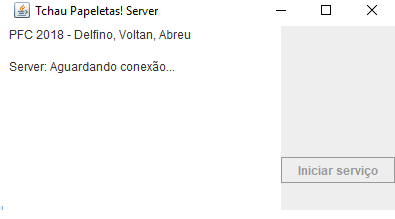
\includegraphics[width=0.5\textwidth]{img/iniciar_conex_o_2.png}   
	\caption{Iniciando serviço: Passo 2}
	\label{fig:figura78}
\end{figure}

\begin{figure}[!ht]
	\centering
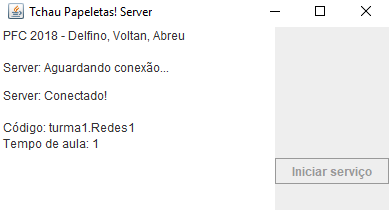
\includegraphics[width=0.5\textwidth]{img/iniciar_conex_o_3.png}   
	\caption{Iniciando serviço: Passo 3}
	\label{fig:figura79}
\end{figure}

\noindent 
